\documentclass[t]{beamer}

\mode<presentation>
{
  \usetheme{default}
  \setbeamertemplate{navigation symbols}{}
  \setbeamertemplate{footline}[frame number]
  \setbeamertemplate{items}[circle]
  \usecolortheme{seahorse}
}

\usepackage[english]{babel}
\usepackage[utf8]{inputenc}
\usepackage{times}
\usepackage[T1]{fontenc}
\usepackage{url}
\usepackage{amsmath}

\parskip=8 pt

\newcommand\topstrut{\rule{0pt}{2.6ex}}
\newcommand\bottomstrut{\rule[-1.2ex]{0pt}{0pt}}
\newcommand\doublestrut{\rule[-1.2ex]{0pt}{3.6ex}}

\newcommand\blue[1]{\textcolor{blue}{#1}}
\newcommand\red[1]{\textcolor{red}{#1}}
\newcommand\gray[1]{\textcolor{gray}{#1}}
\newcommand\smallgray[1]{\textcolor{gray}{\small\it #1}}
\newcommand\prevwork[1]{\smallgray{#1}}

\title[Bienvenu] % (optional, only for long titles)
{Nantes Machine Learning Meetup}
\subtitle{avant-présentation, introductions, etc.}

\author[Abrahamson] {Jeff Abrahamson}

\date[3 novembre 2014]
%{Nantes Machine Learning Meetup, 3 novembre 2014}

% Delete this, if you do not want the table of contents to pop up at
% the beginning of each subsection:
\AtBeginSubsection[]
{
  \begin{frame}<beamer>{Outline}
    \tableofcontents[currentsection,currentsubsection]
  \end{frame}
}

% If you wish to uncover everything in a step-wise fashion, uncomment
% the following command: 
%\beamerdefaultoverlayspecification{<+->}

\begin{document}

\begin{frame}
  \titlepage
\end{frame}

\begin{frame}
  \frametitle{Une mascotte ?}

  \centerline{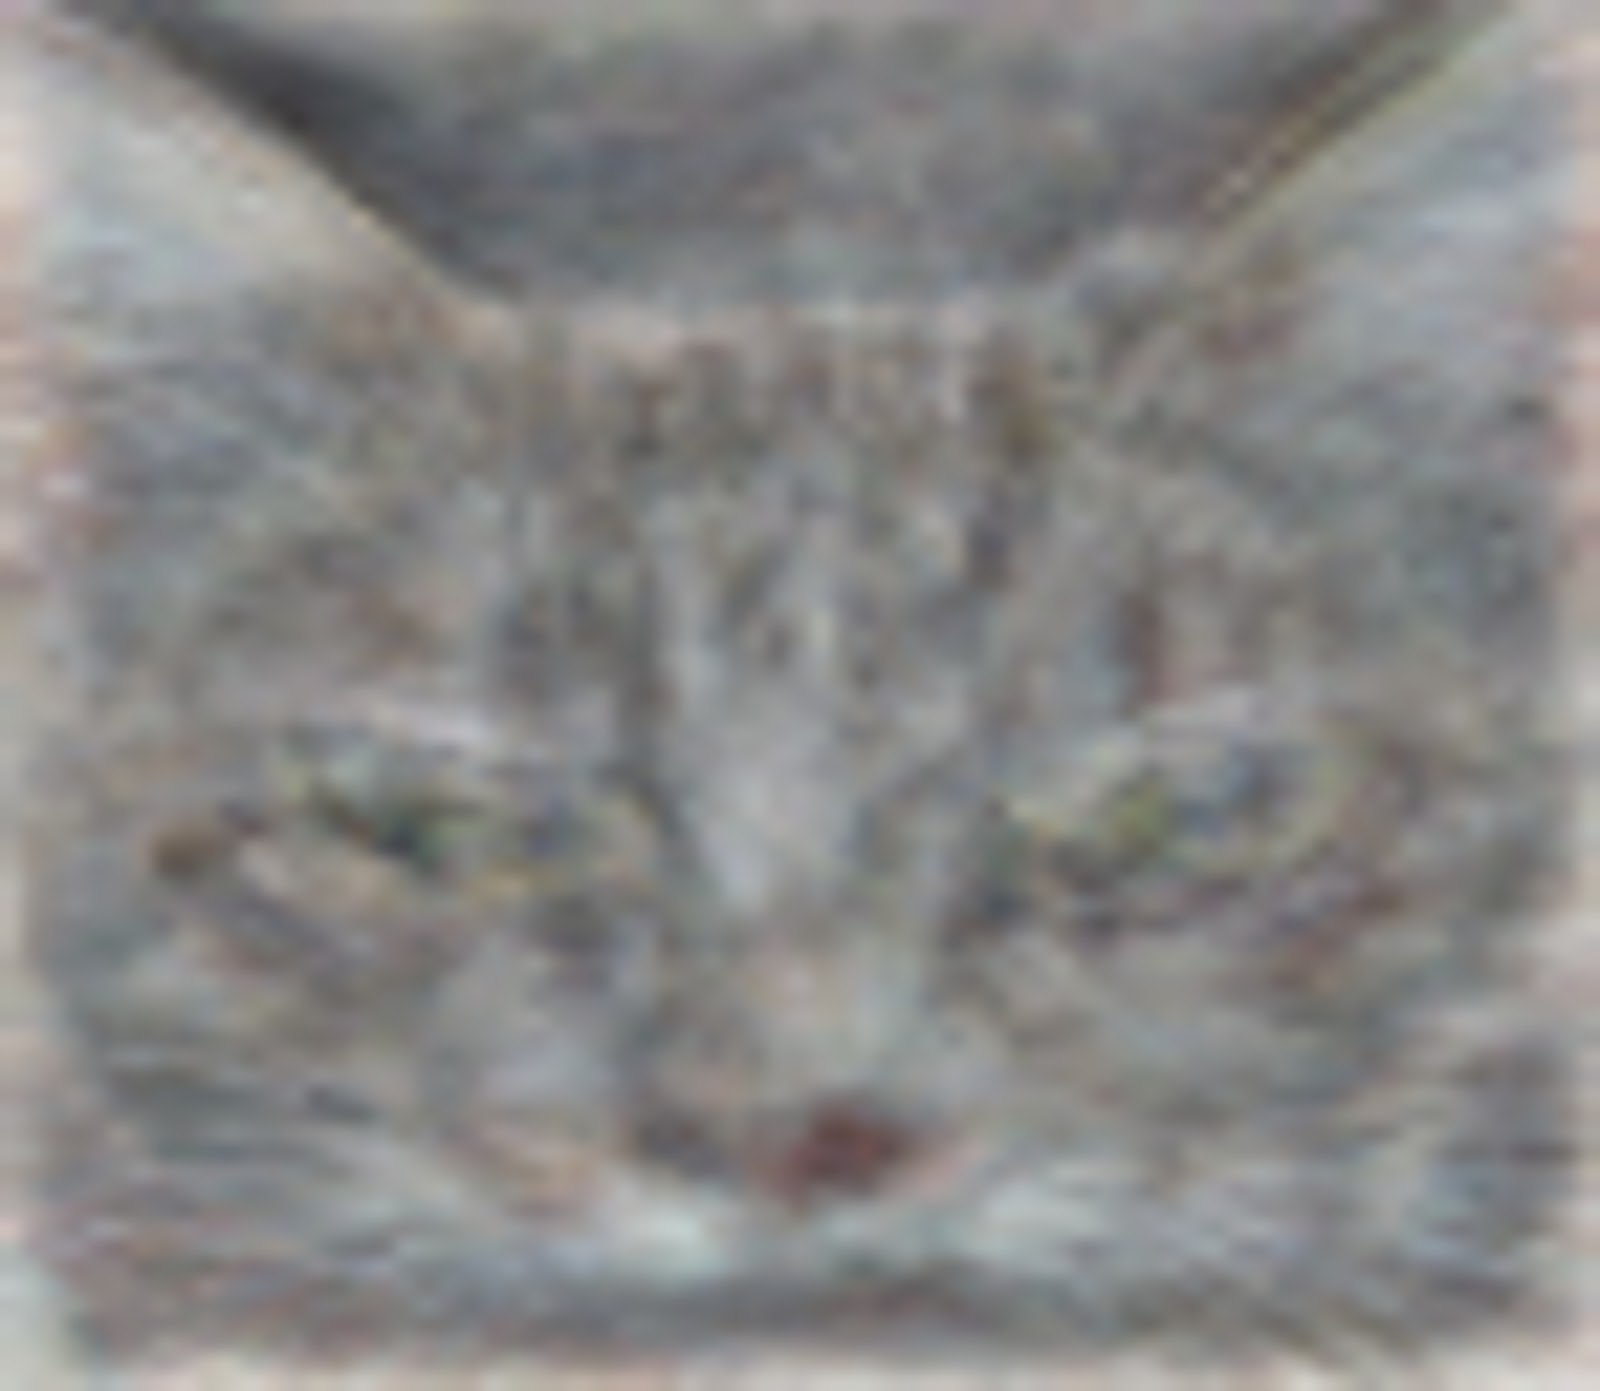
\includegraphics[height=.9\textheight]{cat-detection.jpg}}

  \only<2->{
    \vspace{-7.5cm}
    \centerline{\parbox{.8\textwidth}{Quoc V. Le, Marc’Aurelio Ranzato, Rajat
        Monga, Matthieu Devin, Kai Chen, Greg S. Corrado, \hbox{Jeffrey} Dean,
        and Andrew Y. Ng, \textit{Building High-level Features Using Large
          Scale Unsupervised Learning}, ICML, June 2012.}}
  }
  \only<3->{
    \vspace{4cm}
    \centerline{\parbox{.8\textwidth}
      {\blue{\url{http://research.google.com/archive/unsupervised_icml2012.html}}}}
  }
\end{frame}

\begin{frame}
  \frametitle{Qui nous sommes}
  \begin{minipage}[t]{.88\linewidth}
    \vspace{0pt}
    Nous sommes 47 dans NMLM !
    
    \only<2->{
    \vspace{8mm}
    Pourquoi nous sommes là ?
    \begin{itemize}
    \item Apprendre
    \item Échanges : recherche--commercial
    \item Communauté
    \item Réseautage
    \item \,\dots
    \end{itemize}
    }
    \only<3>{
    \vspace{1cm}
    \parbox{.8\textwidth}{\textit{Et si vous vous êtes inscrit via la Cantine, merci de passer
      à \url{meetup.com}.}}
    }
  \end{minipage}%
  \begin{minipage}[t]{.1\linewidth}
    \vspace{0pt}
    \only<2->{
    
\includegraphics[height=.7\textheight]{registrants.png}
    }
  \end{minipage}
\end{frame}

\begin{frame}
  \frametitle{Introductions éclairs}
  \begin{itemize}
  \item Façon ``lightning talks''
  \item 30 secondes chacun
  \item Go !
  \end{itemize}
\end{frame}

\begin{frame}
  \frametitle{Futurs présentateurs}
  \begin{itemize}
  \item Universitaire (recherche) et industriel
  \item Deux présentations de 30~minutes
  \item Vous ?
  \end{itemize}
  \only<2>{
    \begin{minipage}[t]{.68\linewidth}
      \vspace{0pt} Et diverses :
      \begin{itemize}
      \item Compétitions Kaggle
      \item \url{http://birdsnap.com/}
      \item \url{http://www.datasciencecentral.com/profiles/blogs/could-fake-reviews-kill-amazon}
      \end{itemize}
    \end{minipage}
    \begin{minipage}[t]{.3\linewidth}
      \vspace{0pt}
      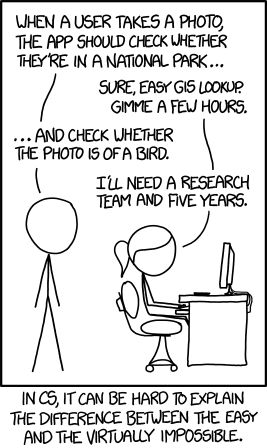
\includegraphics[width=\linewidth]{tasks.png}\\[-1.5mm]
      \blue{\url{xkcd.com/1425}} % Flickr
    \end{minipage}
  }
\end{frame}


\begin{frame}
  \frametitle{Poste (suivra par le meetup)}
  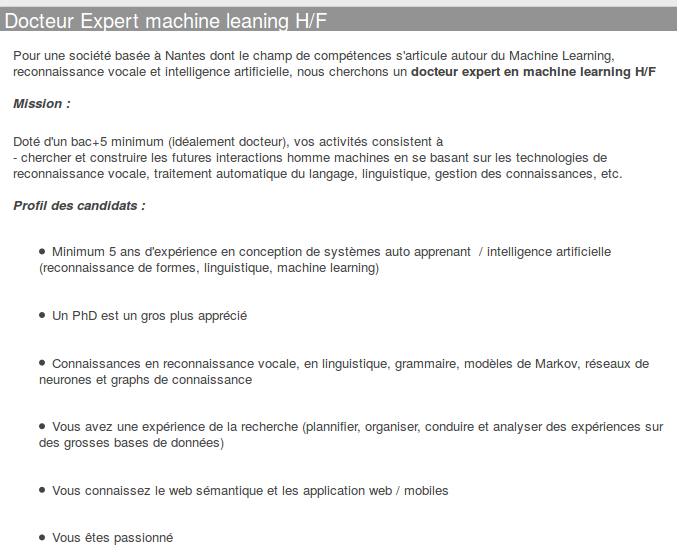
\includegraphics[height=.8\textheight]{externic.png}
\end{frame}

\begin{frame}
  \frametitle{Sponsors}
  Des idées ?
\end{frame}

\begin{frame}
  \frametitle{Ressources après le meetup}
  
  \begin{itemize}
  \item Présentations sur github
  \item Références : suivre sur le meetup
  \item Tout ce qui est intéressant
  \item Annonces diverses
  \end{itemize}
\end{frame}

\begin{frame}
  \frametitle{Présentateurs}

  \vspace{1mm}
  
\includegraphics[scale=.5]{dictanova.png}

  \begin{itemize}
  \item Damien Raude-Morvan
  \item Sebastián Peña Saldarriaga
  \end{itemize}
\end{frame}


\end{document}
